\chapter{Elméleti alapok, szimulációs technikák}
\label{chapt:theoretical_intro}

\begin{comment}
Tehát a kövezezőkről van itt szó:
1.
Alklamazott statisztikus eloszlások és a Gamma függvény:
 - ami a cimben szerepel, ez igazából már kész is van

2. 
Törés és statisztikus fizika, vagy szilárd testek törésének statisztikus fizikai aspektusai
	Ezt valahogy a zoli a gábor a geri és a cikkek alapján kéne összeszedni. Majd meglátjuk mennyire lehet.
	-hatványfüggvények jelentősége 
	-fázisátalakulások
	-univerzalitás

3.
Törés modellezési lehetőségei:
 - egy kis bevezető miért érdekes a törés vizsgálata, habár az introduction is pont erről szól.
 - Fragmentáció:
 		Általános elméleti bevezető a fragmentációról, illetve néhány kép ami bemutat néhány
 		fragmentációs folyamatot. Esetleg ábra a hatványfüggvény eloszlásról, könyvből kell kivenni
 		megnézem majd Gábor dolgozatát. Továbbá kellenek még majd referenciák
 - FBM:
 	  A zoliéhoz hasonló bevezetése az általános modellnek. Példákat mutatva, kvázi irodalmat
 	  áttekintve vele, hogy mire is lehet még használni ezt a modellt.
 	  Ábrák:
 	  -LLS hatványfüggvény
 	  -GLS hatványfüggvény
 	  -Constitutive görbe
 	  
 	  Érdemes lenne még az FBM esetében fontos jellemzőkről beszélni:
 	  -lavina méret eloszlás
 	  -Állapot egyenlet, a megyúlás feszültés ábra
 	  -

4.
Szimulációs technikák 
	- Molekuláris dinamika:
		 Itt nyilván a módszer jellemzőit írom le, példát hozva a kölcsönhatásokra, de igazából nem kell
		 annyira belemenni a példákba, mert a későbbi fejezetben részletesen ismertetek egy modellt amit használtunk
		 
	- Szálköteg modell szimulációja
 
	-
\end{comment}

Ebben a fejezetben rövid áttekintését szeretném adni a dolgozatban felhasznált matematikai, statisztikus fizikai és számítógépes fizikai fogalmaknak, modelleknek és szimulációs technikáknak.
A doktori munkám eredményeit képező módosított modelleket a megfelelő fejezetben fejtem ki.


\section{Alkalmazott Statisztikus eloszlások és a Gamma függvény}
\label{sec:functions_gamma}
A dolgozat célkitűzése rendezetlen anyagok szimulációs vizsgálata. Ez a rendezetlenség az általam vizsgált rendszerekben a makroszkópikus testet felépítő, mezo- illetve mikroszkópikus elemek jellemzője. A munkám során alkalmazott két fajta modellben ez a következő képen jelenik meg. A fragmentációs modell esetében (lásd \ref{chapt:md}) a rendszert felépítő - molekuláris dinamikai értelemben vett (lásd \ref{subchapt:md}) - atomi elemek közötti kohéziós kölcsönhatást reprezentáló rudak törési küszöbeiben, míg a szálkötegmodell (lásd \ref{subchapt:fbm}) esetében a szálak szakítószilárdságában jelenik meg. A modellben és a szimulációs programban ezeknek a jellemzőknek egy-egy valószínűségi változót feleltetünk meg, amit egy előre definiált valószínűségi eloszlás jellemez.

A dolgozatban két eloszlásnak lesz fontos szerepe. Az egyenletes eloszlásnak és a két paraméteres Weibull eloszlásnak.

\subsection{Egyenletes eloszlás}
A test valamilyen váltakozó, folytonos valószínűségi változóval \cite{distribution_valseg} leírható jellemzőjének az eloszlása egyenletes eloszlást követ egy $(a,b)$ intervallumon, amennyiben a mintavételezéssel kapott sűrűségfüggvénye
\begin{equation}
	f(x)= 
	\begin{cases}
		\D \frac{1}{b-a}, & \mbox{ ha } a\leq x\leq b \\
		0, & \mbox{egyébként.}
	\end{cases}
\end{equation}
alakú.
Egyenletes eloszlást akkor használunk amennyiben az egyes események bekövetkezési valószínűsége azonos, pontosan ezért akkor is érdemes első közelítésnek használni amikor nincsenek ismereteink az adott véletlenszerű rendszerjellemzőről, mivel így egyetlen értéket sem tüntetünk ki, mint az a \ref{fig:unif_weib_distrib}. ábra bal oldalán látható. Az egyszerű függvény alak miatt, amennyiben a modellünket analitikusan szeretnénk kezelni akkor is érdemes lehet ezt az eloszlást használni.

Van egy technikai előnye is ennek az eloszlásnak, mivel a számítógépen különféle algoritmusokkal elég jó minőségű egyenletes eloszlású pszeudovéleteln számsorokat lehet generálni, amit felhasználva, a transzformációs módszer segítségével \cite{comphys_woolfsonpert1999} tetszőleges eloszlású pszeudovéletlen értékeket előállíthatunk.

\subsection{Weibull eloszlás}

A Weibull eloszlás egy tapasztalati eloszlás amelyet részleteiben először Waloddi Weibull írt le 1939-es munkájában \cite{distributions_weibull1939}, ami akkor a tudományos közélet számára többé kevésbé ismeretlen maradt, így a cikk átírt 1951-es változata óta terjedt el szélesebb körben a használata \cite{distributions_weibull1951}, habár magát az eloszlást Maurice Fréchet fedezte fel 1927-ben \cite{distributions_weibull_frechet1927} és 1933-ban alkalmazták először, amikor szénpor  részecskék méreteloszlását írták le vele \cite{distributions_weibull_rosin1933}. 

Ennek az eloszlásnak a felhasználásától függően létezik több paraméteres változata is, a munkám során én a kétparaméteres Weibull eloszlást használtam amelynek eloszlásfüggvénye

Első lépésben az egyszerűsége és analitikus kezelhetősége miatt feltételezhetjük, hogy a vizsgált rendszerünkben a rendezetlenség egyenletes eloszlás formájában jelenik meg. 
Azt mondjuk, hogy egy mennyiség egyenletes eloszlású \ref{distribution_valseg}, az $(a,b)$ intervallumon, pontosabban egy folytonos valószínűségi változó egyenletes eloszlású az $(a,b)$ intervallumon, amennyiben az $F(x)$-el jelölt eloszlásfüggvénye a következő alakú:
\begin{equation}
	F(x)= 1 - e^{-(\frac{x}{\lambda})^m},
\end{equation}
ahol a $\lambda$ egy skálaparaméter ami a függvény $x$ tengely menti eltolásáért felelős, míg az $m$ az alakparaméter aminek a segítségével az eloszlás rendezetlenségét lehet kontrollálni. Az m növelésével az eloszlás rendezetlensége csökken, mint azt a \ref{fig:unif_weib_distrib} ábra jobb oldalán láthatjuk. Minél nagyobb $m$ értéke, annál több érték öszpontosul egy a $\lambda$-tól föggő érték körül.
\begin{figure}
%[!htb]
\label{fig:unif_weib_distrib}
\caption{A bal oldali ábrán az egyenletes eloszlás sűrűségfüggvénye látható, míg a jobb oldali ábrán az $m$ alak paraméter hatása a Weibull eloszlás rendezetlenségére.}
\centering
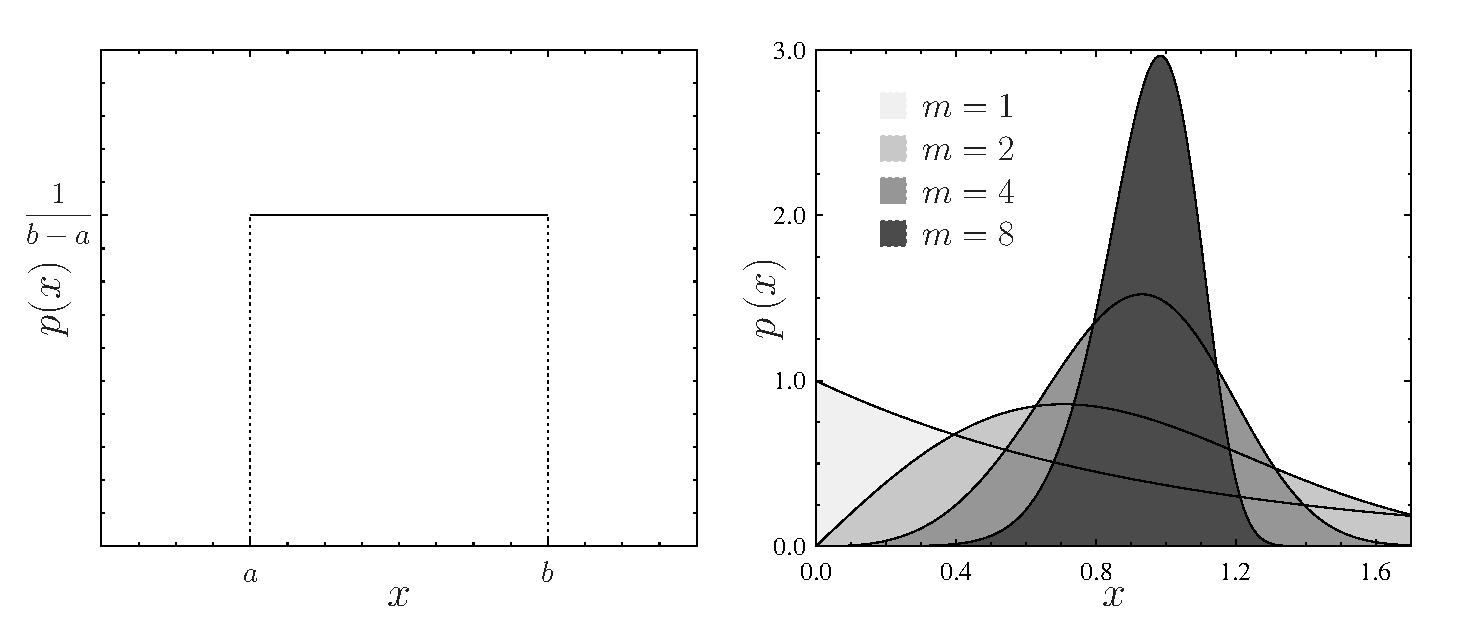
\epsfig{bbllx=-1,bblly=503,bburx=684,bbury=794,file=chapters/pics/introduction/unif_weib.eps,width=12cm}
\end{figure}

		
\subsection{Az Euler féle Gamma függvény}
\cite{distribution_stat2000}
	A Gamma függvényre a szálköteg modell doktori munkám során kibővített modelljének egy határesetében megadható analitikusan meghatározható hatványfüggvény exponens meghatározásában lesz szerepe. A Gamma függvényt a következő alakban írhatjuk fel:	
	\begin{equation}
		\Gamma\left(s\right)=\int_0^{\infty} \! t^{s-1}e^{-t} dt,
	\end{equation}
amiből parciális integrálással adódik, hogy amennyiben az $s$ valós része nagyobb mint $1$ akkor a Gamma függvény a következő alakot veszi fel:
	\begin{equation}
		\Gamma(s)=(s-1)\Gamma(s-1),
	\end{equation}
emiatt ha $n$ pozitív egész akkor $\Gamma(n)=(n-1)!$ amivel a faktoriális általánosításának tekinthető.


	Ebben a részben írnom kell a törés és a statisztikus fizika kapcsolatáról, valami rövid tömör bevezetőt a fázisátalakulásokról kapcsolatukról a hatványfüggvényekkel, kritikus jelenségekkel skálatörvényekkel. 
	A szilárdtestek törésének vizsgálati technikáiról egy fejeztet értem ezalatt valami a molekuláris dinamikáról, valamit a szálköteg modellről. Fragmentációs folyamatok, illetve a kvázisztatikus terhelés, ahol statikus állapotokon keresztül vizsgáljuk a törés mechanizmusát. Két féle modell és két féle szimulációs technika

A fejezetben szó lesz a hatványfüggvényekről, a fázisátalakulások elméletének érintőleges tárgyalásáról, a szilárdtestnek törésének statisztikus aspektusairól.
A munkám során szemcsés és erősen rendezetlen anyagok viselkedését vizsgáltam. Az anyagok rendezetlenségét a modellekben valamilyen valószínűségi eloszlásfüggvény segítségével ragadtuk meg. Ezért szentelek itt egy rövid fejezetet a használt eloszlások ismertetésre. 

\section{Törés modellezési lehetőségei}

\subsection{Fragmentáció}

\subsection{A szálköteg modell (FBM)}
Ide le akarom írni a rengeteg példát amit ezzel a modellel el lehet érni, a saját kiterjesztésünket pedig majd kifejtem lent az FBM-hez tartozó fejezet részen.
Írni egy pár szót a változó távolságú kcshról, meg a korlátozott terhelés eloszlásról, meg a rengeteg eredményről, aztán arról, hogy hogyan sikerült aszfaltot, vagy forgatónyomatékot kifejteni képes rudakat is modellezni ezzel a nagyon egyszerű modellel. 
Az elemek közötti kölcsönhatás hatótávolságától függő kölcsönhatás. 
A modell kapcsolata más modellekkel, a modellel vizsgált mennyiségek, jellemzők és az abból levonható következtetések...

\section{Szimulációs technikák}
A különféle fizikai rendszerek mechanikai deformációjának, sérüléseinek, fragmentációjának vizsgálatára az évek során több szimulációs technika is született. Amennyiben a vizsgálni kívánt jelenség a kontinuum fizika tárgykörébe tartozik akkor általában valamilyen véges elem módszerre (FEM)\cite{comphys_woolfsonpert1999} épülő, ha a jelenség modellje diszkrét leírást tesz lehetővé (atomok, molekulák, szemcsés anyagok) akkor általában valamilyen diszkrét elem módszerre (DEM), vagy molekuláris dinamikára (MD) épülő technikával szokás szimulálni a folyamatot. Munkám során a fragmentációs folyamatot molekuláris dinamikai szimuláció segítségével vizsgáltam. Több a kereskedelmi forgalomban kapható, vagy nyílt forráskódú szoftver is létezik, amelynek testreszabásával elvégezhetjük a vizsgálatainkat. A kíváncsiságomtól vezérelve az évek során két nyílt forráskódú programcsomaggal is megismerkedtem. Az egyik az ausztráliai Queenslandi Egyetem eSys-Particle csomagja, a másik a Sandia National Lab által támogatott, és részben az ott dolgozók által fejlesztett LAMMPS. A saját munkámhoz egy a témavezetőm által írt, és a feladatnak megfelelően általam továbbfejlesztett molekuláris dinamikára épülő kódot használtam. 

A fentebb ismertetett szálköteg modell vizsgálatához szintén saját kódot fejlesztettem, aminek segítségével a lentebb ismertetésre kerülő modell mellett számos egyéb modellváltozatot is teszteltünk a kutatás során, illetve a terület mára klasszikusnak tekinthető eredményeit a kód validációja gyanánt újra előállítottuk. 

Mind a két modellezési technika jól párhuzamosítható, habár a szálköteg modell esetén erre nem volt szükség, mert a szimulálható rendszerméret így is a $10^5$ - $10^6$ nagyságrendbe tartozott, meglehetősen rövid, legfeljebb órákban mérhető futásidő mellett. 
Mivel a később ismertetésre kerülő modellből látható, hogy a rendszerben csak rövidtávú kölcsönhatások lépnek fel, ezért a szimulált rendszert feloszthatjuk és az egyes részeket külön magokhoz rendelhetjük. Mind a három - MPI, OMP, CUDA/OpenCL -  a számítógépes klaszterekben elterjedt párhuzamos számításokhoz használt technika jól alkalmazható ebben az esetben. 
A fragmentációhoz használt modell egy módosított, dinamikus repedést vizsgáló \cite, a dolgozatban nem ismertetett változatának implementációja során volt lehetőségem OMP és CUDA alapú implementációk kipróbálására.

\section{A molekuláris dinamikai módszer}
Diszkrét elemekből felépülő a Newton féle mozgásegyenletekkel leírható, a klasszikus mechanikára épülő determinisztikus rendszereket vizsgálunk molekuláris dinamikai szimulációval. Ezekben a rendszerekben sztochasztikus jellemzők többnyire csak valamilyen rendszerjellemző, vagy kezdeti feltétel meghatározásakor vannak jelen.

A módszert az 1950-es években fejlesztette ki Alder és Wainwright \cite{md_firstpub} óta használják anyagok vizsgálatára, ahol a rendszert alkotó részecskék és az elemek között fellépő kölcsönhatások miatt nincs mód analitikus számításokra.

A molekuláris dinamika alapötlete egybecseng a determinizmus filozófiai nézetével. Laplace gondolatkísérletében úgy gondolta, hogy ha létezne egy olyan mindenható lény aki pontosan ismeri a világ aktuális állapotát és az elemek között fennálló fizikai törvényeket, akkor pontosan meg tudja mondani a világ állapotát bármely időpontban. A kvatnum és káoszelmélet megjelenése óta  tudjuk, hogy nem csak a véges ismeret és a véges számoló kapacitás áll annak az útjában, hogy a világ viselkedését pontosan előjelezzük.

\subsection{A módszer fizikai háttere}
Amikor egy molekuláris dinamikai kód megírásához kezdünk akkor először a vizsgálni kívánt rendszer mikroszkópikus modelljét alkotjuk meg, amelynek elemei a rendszert alkotó részecskék, a kölcsönhatások és a mozgásegyenletek\cite{md_szamfiz}. Miután ezeket meghatároztuk, meg kell fogalmaznunk a rendszer határfeltételeit, ki kell választanunk valamilyen numerikus módszert a mozgásegyenletek megoldására, figyelembe véve a szimulálni kívánt folyamat releváns időskáláját
\subsubsection*{Részecske} 
Meg kell határoznunk azt, a rendszer vizsgálata szempontjából fontos legkisebb építőelemet, amit már belső szerkezet nélkülinek tekinthetünk, azaz a vizsgált jelenség szempontjából irreleváns, hogy a részecskén belül mi történik. Ezek az elemek határozzák meg a rendszer mikroszkópikus szabadságfokait. Például szemcsés anyagok vizsgálatakor az anyag szemcséit tekintjük részecskének annak ellenére, hog ezeket Avogadro-számnyi atom alkotja.
\subsubsection*{Kölcsönhatások} 
Miután megállapítottuk, hogy melyek lesznek a rendszer építőkövei, meg kell határoznunk, a részecskék közötti kölcsönhatásokat. Mivel modellalkotásról van szó, ezért nyilván nem fogunk kitérni minden lehetséges kölcsönhatásra, csak azokra amelyek a vizsgált folyamat szempontjából relevánsak. Ezek a kölcsönhatások lehetnek taszító vagy vonzó jellegűek, esetleg mindkettő a két részecske távolságának a függvényében. Lehetnek nagy hatótávolságúak, mint például a tetszőleges két tömeggel rendelkező részecske, test között fellépő gravitációs erő, vagy két töltéssel rendelkező részecske között fellépő Coulomb erő. Ilyen típusú kölcsönhatások esetében - különösen ha azok nem négyzetes, hanem valamilyen magasabb kitevőjű fordított arányosságban állnak a két részecske távolságával - optimalizációs céllal meg szokás adni egy úgynevezett vágási távolságot, vagy vágási sugarat aminél nagyobb távolságban adott kölcsönhatás hatására, a két részecske között fellépő erő nagysága $F=0$. Ilyen kölcsönhatás például a két gázmolekula kölcsönhatását leíró Lennard-Jones potenciál, aminek képlete:
\begin{equation}
\displaystyle
\vec{F}(\vec{r}_{ij})=-\nabla V(\vec{r}_{ij})=\frac{24\epsilon}{r_{ij}}\left[2\left(\frac{\sigma}{r_{ij}}\right)^{12}-\left(\frac{\sigma}{r_{ij}}\right)^{6}\right]\vec{r}_{ij}^{0},
\end{equation} 
ahol $\epsilon$ a potenciálgödör mélységét míg $\sigma$ a potenciál zérushelyét adja meg. Kihangsúlyozom, hogy a mennyiségek nem keverendők össze a szálköteg modellnél alkalmazott azonos jelű mennyiségekkel. 

A kölcsönhatás lehet rövid hatótávolságú is, ennek határesete amikor két test csak akkor fejt ki erőt egymásra amennyiben közvetlenül érintkeznek.
Rövid hatótávolságú kölcsönhatásra példa a nedves közegben lévő homokszemcsék között fellépő kohéziós erő. Ahelyett, hogy ezt a valóságnak megfelelően  hidrogén kötéssel, vagy Van der Walls erővel írnánk le, a modellünkben egyszerűsítő feltevésként tekinthetjük úgy mintha a két homokszemcsét egy rugó kötné össze, a következő viszonylag egyszerű erőtörvénnyel:
\begin{equation}
\vec{F}_{A\rightarrow B}=-D(r_{0}-r_{AB})\frac{\vec{r_A}-\vec{r_B}}{|\vec{r_A}-\vec{r_B}|},
\end{equation}
ahol $r_0$ és $r_{AB}$ a rugó nyugalmi és aktuális hossza, a $D$ pedig a rugó keménysége. Végül természetesen majd a szimulációs eredményeink kísérletekkel való összevetése dönti majd el, hogy élhetünk-e a fentihez hasonló egyszerűsítő feltevésekkel.
\subsubsection*{Mozgásegyenletek} 
Végül az előzőek ismeretében felírjuk a vizsgálni kívánt rendszer elemeire azok klasszikus mechanikai mozgásegyenleteit. Ezek egy másodrendű differenciálegyenlet rendszert alkotnak, amit csak a legegyszerűbb eseteben lehet analitikusan megoldani. A számítógépes fizikában használt numerikus módszerek segítségével az ilyen egyenletekrendszerek közelítő megoldását képesek vagyunk meghatározni, és ezzel komplex, összetett viselkedésű rendszerek vizsgálatát végezhetjük el. Végül a rendszer makroszkópikus jellemzőit a részecskék jellemzői feletti átlagolással határozzuk meg. 

Tegyük fel, hogy a vizsgált rendszer $N$ darab tömegpontból épül fel. Ebben az esetben a mozgásegyenlete a következőnek adódik:
\begin{equation}
m_{i}\ddot{\vec{r}}_{i}=\vec{F_i}(\vec{r}_1,\vec{r}_2,\dots,\vec{r}_N),
\end{equation}
ami pedig egy $N$ egyenletből álló csatolt differenciálegyenlet rendszer, aminek a megoldásához meg kell adnunk a kezdőpillanatbeli $\vec{r}_i(t_0)$ hely és $\vec{v}_i(t_0)$ sebesség vektorokat.

Az így meghatározott rendszer időfejlődése determinisztikus, sztochasztikus véletlen elemeket, csak a kezdeti feltételek meghatározásában tartalmaz. Előfordulhat az is, hogy a rendszert alkotó részecskék mozgásának eredményeként bekövetkező esemény sztochasztikus jellegű, persze ettől függetlenül két egymást követő lépés még teljes mértékben determinisztikus. 

\subsubsection*{Peremfeltételek}
Mivel a legtöbb ha nem minden szimuláció esetében a valóságnak csak egy erősen leegyszerűsített modelljét szimuláljuk, ami általában nem csak a kölcsönhatások idealizálásában ha nem a vizsgált rendszer méretében is megmutatkozik. A számítógépek és az algoritmusok véges - habár egyre növekvő - számítókapacitásának következtében a rendszerünkben valamilyen peremfeltételeket vagyunk kénytelenek megadni.
Amennyiben a vizsgálni kívánt rendszer ideális esetben Avogadro számnyi elemet 
Peremfeltételekre több okból is szükség van. Amennyiben a részecskéink valóban molekulákat vagy atomokat szimbolizálnak, akkor ideális esetben Avogadro számnyi 
Bizonyos vizsgált esetekben fontosak a felületi effektusok, erre példa ha azt vizsgáljuk, hogy zárt tér hatására hogyan viselkedik  és ilyenkor definiálnunk kell azt a teret amiben a részecskék mozognak. Ideális esetben amennyiben 


\subsection{Numerikus integrálási módszerek}
A molekuláris dinamikában a megoldandó feladat a rendszert alkotó elemek időfejlődését leíró mozgásegyenletek megoldása. Ez matematikailag egy közönséges másodrendű differenciálegyenlet megoldását jelenti, amelyet zárt alakban csak a legegyszerűbb esetekben tudunk megoldani. A szimulációk esetén ezek az egyenletek gyakran csatoltak, így megoldásukra csak közelítő módszereket használhatunk. Többféle numerikus módszert fejlesztettek ki az évek során, mindnek megvan a maga előnye és hátránya.

Többé kevésbé igaznak tekinthető az az állítás, hogy minél pontosabb egy közelítő eljárás, annál nagyobb a számításigénye, így a szimulációt készítő kutatónak mindig mérlegelnie kell, hogy mennyit áldoz fel a pontosságból a sebesség oltárán azért, hogy az eredményei kivárható időn belül megszülessenek. Habár a számítástechnika fejlődésének köszönhetően azt gondolhatnák, hogy egyre kisebb kompromisszumra kényszerülünk, azonban egyre nagyobb és nagyobb rendszereket, egyre összetettebb kölcsönhatásokat igyekszünk modellezni, így a kutatóknak a belátható jövőben is szembe kell nézniük ezzel a problémával.

Mint minden kísérlet, így a számítógépes szimuláció is hibával terhelt. Az esetleges bemeneti adatok mérési hibája mellett a számítógép technikai megoldásai és maguk az algoritmusok újabb hibákkal terhelik az eredményeket amit mindig szem előtt kell tartani. Minden a számítógépen, lebegőpontos számokkal végzett számítás néhány szerencsés esettől eltekintve a számábrázolás véges pontossága miatt hibával terhelt \cite{nummat_gisbert,nummat_vertse}. 

Egy egyszerű kezdő trükk ennek a hibának a csökkentésére, hogy a szimulációban olyan mértékegységeket használunk amelyben a releváns mennyiségek nem lesznek túl kicsik, ezzel csökkenthetjük a kerekítésből eredő


\subsubsection*{Euler}

\subsubsection*{Verlet}

\subsubsection*{Runge-Kutta}

\subsubsection*{Prediktor-Korrektor}

\subsection*{Implementációs kérdések}

\section{Törés és statisztikus fizika}



	\subsection{Hatványfüggvények és jelentőségük}
	Az elmúlt évek tapasztalata alapján a hatványfüggvények igen fontos helyet foglalnak el a különféle
	fizikai rendszerek vizsgálatakor. Sok cikk konkluziójában olvashatunk arról, hogy kimutatták hogy az adott vizsgált rendszer adott jellemzői hatványfüggvény jelleget mutatnak, esetleg adott jellemző követi a Zipf törvényt, vagy Pareto eloszlást követ. Ezek a fogalmak mind ugyanarra utalnak. Ezen eredmények jelentősége abban rejlik, hogy a hatványfüggvény jelleg a tapasztalatok szerint egyéb rendszerjellemzőkre is utal. Kapcsolatokat találhatunk látszólag teljesen különböző folyamatok között, ami a folyamatok mélyebb megértésében segítheti a kutatót. 
	
	Az egyik ok ami miatt nagy jelentőséggel bírnak a hatványfüggvények, mert univerzalitási osztályokat jelölhetnek. Az univerzalitási osztályok jelentősége, hogy.. KIFEJTENI... A fragmentáció jelenségének tárgyalásakor több példát is mutatok majd az univerzalitásra, továbbá a szálkötegmodellek tárgyalásával kapcsolatos munkám egy új univerzalitási osztály vizsgálatához kapcsolódik. 
	
	Hatványfüggvény jelleget követő jellemzőkről tudható, hogy nincs releváns méretskálájuk, ami azért érdekes, mert....
	
	A kutatók az elmúlt évtizedek munkája eredményeként a természet legkülönfélébb jelenségeinél fedezték fel a hatványfüggvény viselkedést, és vontak le ennek köszönhetően hasznos következtetéseket. A már említett fragmentáció mellett, a városok méreteloszlása, az internet routereinek a kapcsolatszámai, a különféle folyóiratok hivatkozási hálózata, a földrengések mérete illetve a holdi kráterek mérete (ami egyébként a fragmentáció folyamatához köthető).
	
	Szó lesz ebben a fejezetben a hatványfüggvények "vadászatának" technikai kérdéseiről is \cite{}. 
	A hatványfüggvények hajszolásának meg vannak a maga veszélyei. Két alapvető technikai problémára vezethetjük vissza ezeket. Az egyik magának a függvénynek az előállítása mintavételezéssel, különféle dobozolási technikákkal. Amelynek a hátulütője, hogy a véges mintának köszönhetően a függvény farka általában igen zajos. Lásd az ÁBRÁT. 
	
	A hatványfüggvények 
	
	A hatványfüggvényeket a fázisátalakulások elméletében is felhasználjuk, ez a következő fejezet tartalmazza. További kapcsolódásai a 
	
	\begin{itemize}
		\item hatványfüggvények fittelése
		\item fittelési pontatlanságok
		\item 
	\end{itemize}
	\subsection{Fázisátalakulások elmélete}
		A kritikus jelenségek elmélete nagyon fontos területe a fizikának
		A fázisátalakulások jelenségével mindannyian találkozhattunk már. A legnyilvánvalóbb formája amikor valaminek a halmazállapota változik meg. A leghéztköznapibb példa erre a víz halmazállapotváltozása
		A fázisátalakulás fő jellemzője, hogy a vizsgált rendszernek az úgynevezett kontroll paraméter egy speciális, kritikus értékénél megváltoztatják a viselkedésüket. Az elmélet egy másik fontos jellemzője az úgynevezett rendparaméter. Ennek függvényében beszélhetünk rendezett és rendezetlen 

\section{Fázisátalakulások amire szükség van}

%%%%BLABLA
Habár a fázisátalakulások elméletét egzakt módon csak a termodinamikai határesetben alkalmazhatjuk, mondjuk ez általában igaz a statisztikus fizikára, mivel statisztikai eszközökkel operál ezért kellően nagy rendszerméret és/vagy minta, kísérlet, teszt szükséges ahhoz, hogy a kapott eredmények értelmezhetőek az elméleti eredményekkel összevethetőek legyenek. A termodinamikai határeset létezésének egyik feltétele, hogy a vizsgált rendszerben a kölcsönhatási potenciálok távolság függésének kitevője nagyobb legyen mint a vizsgált rendszer dimenziója, ezek alapján Coulomb vagy a gravitáció kölcsönhatások $1/r$ típusú potenciálja mellett három dimenzióban nem létezhetne a termodinamikai határeset, azonban ezek a kölcsönhatások egy sok részecskés rendszer esetében általában árnyékolják egymást, ezért a hatásnak exponenciális lecsengése lesz, ami pedig már lehetővé teszi a termodinamikai határeset létezését. Az általam vizsgált rendszerek habár véges méretűek - a szálköteg modell esetén ezt a korlátozást a periodikus határfeltétel bevezetésével igyekeztünk ellensúlyozni - de a kölcsönhatások szigorúan rövid hatótávolságú párkölcsönhatások, ez alól kivételt képez a szálköteg modell GLS változata, mivel az egy átlagtér modellnek felel meg, de az irodalom...

Fázisátalakulások osztályozása:
Többféle osztályozás is létezik az egyik az Ehrenfest féle, ami a termodinamikai potenciál deriváltjainak változása alapján osztályozza a fázisátalakulásokat (referencia keresés Gulácsi könyvében), a későbbiekben kiderült, hogy például a termodinamikai potenciál másodrendű deriváltjai nem ugrást szenvednek, hanem divergálnak. Ez a divergencia jóval pontosabban írja le a fizikai eseményeket, mivel ezek a fázisátalakulások általában valamilyen térbeli rendezettség, korrelációs hossz illetve egyéb jellemzők változásával járnak együtt.

Egy rendszer fázisátalakulásainak vizsgálatához a dimenzió paramétert fixálnunk, ugyanis a dimenzió alapvetően befolyásolja a folyamatot, ezt fontos figyelembe venni a dolgozatban bemutatott eredmények esetében is. 


%%%%BLABLA vege


A fázisátalakulás elmélete egy nagyon összetett közel egy évszázada aktívan kutatott terület, ami mind a mai napig tartogat megoldatlan problémákat. A jelenség leghétköznapibb speciális esete amikor a fázisátalakulás halmazállapot-változással jár együtt. Általános esetben - kicsit pongyolán megfogalmazva - fázisátalakulásról beszélünk amennyiben a vizsgált rendszer valamilyen mennyiségi vagy minőségi jellemzői hirtelen változáson mennek keresztül egy meghatározott rendszerjellemző folytonos változtatásának a hatására. Ezt a folytonosan változtatott jellemzőt kontroll paraméternek, azt az értéket ahol a változás megtörténik a kontroll paraméter kritikus értékének nevezzük. Az elmélet alapján a rendszer rendparaméterének nevezzük azt a rendszerjellemzőt ami a kontroll paraméter kritikus értéke alatt egyenletesen nulla, míg a kritikus érték felett valamilyen véges érték. 
\begin{equation}
 rend(T_c)=0  T<T_c
 rend(T_c)>0  T>=T_c
\end{equation}
 REF(Stauffer, Complexity, criticality, Stanley, etc...)
A változáson átmenő paraméter a rendszer rendparamétere 
A fázisátalakulásoknak több osztályozása ??? is létezik

Azt a tartományt amikor a kontroll paraméter közel van a kritikus értékéhez kritikus tartománynak nevezzük. A rendszereket a kritikus állapotban jellemezhetjük úgynevezett nevezetes vagy kritikus exponensekkel. (Volt ido amikor azt gondoltak, hogy itt is található egy univerzális konstans érték, legalábbis a kezdetben vizsgált jelenségek erre utaltak Stanley 6 gazfolyadek, ennél azonban véleményem szerint még fontosabb eredménye lett mivel habár különböző exponensek léteznek de az egyes jelenségek az eddigi ismeretek alapján univerzalitási osztályokba sorolhatók a kritikus exponenseknek köszönhetően... )

Életbeli példák: gáz-folyadék fázisátalakulás

Fázisgöbe:

Ejtek itt néhány szót a fázisátalakulások perkolációs interpretációáról, mivel a munkám során a vizsgált témák között előfordult...

Perkolációs exponensek - klaszterek jellmezői, fázisátalakulás a fragmentációban errol is irni a  kisérlet magyarázatán túl, továbbá tovább vinni ezt a vonulatot az fbm-re persze ott még inkább erről van szó, kritikus jelenségek, fázisátalakulás....
	
\section{Szilárd testek törésének statisztikus aspektusai}



\section{Általános elméleti ez megaz}
Időskála. Minden fizikai folymathoz tartozik valamilyen releváns időskála amennyiben az adott rendszert szignifikánsan hosszabb vagy rövidebb időintervallumon vizsgáljuk akkor az adott jelenségnek nem lesz releváns hatása a rendszer viselkedésére. Általánosan azt mondhatjuk hogyha a vizsgált időintervallumban a vizsgált jellemzők szempontjából a rendszer nem változik akkor azt mondhatjuk, hogy termodinamikai egyensúlyban van. (az időskálák szétválását jól szemlélteti egy tejjel felöntött, megkavart, kihűlt majd elpárolgott csésze tea folyamatainak releváns időskáláinak logaritmikus skálán való ábrázolása: diffúzió/keverés, lenyugvás, kihűlés, elpárolgás)


\section{Szimulációs módszerek technikák}
Molekuláris dinamika, rácsomdellek, általános szimulációs leírása, mig a konkrét modell változatokat részletesen leírhatom ott ahol szó lesz róluk.




%Coefficient of variation alapján használhatjuk a uniformot, pont azért ami a CV jellemzője, ami dimenzió nélküli (képlete szórás négyzer per várható érték, vagy szórás per várható érték, RMSD mértékegység mentes, csak pozitív értékű nem 0 várható értékű valségi változók és hozzájuk tartozó eloszlások esetén lehet értelmesen interpretálni az értékét, továbbá 

%	Érdemes megjegyezni: Stirling képlet: $n!\simeq \left(\frac{n}{e}\right)^n$
%A pontos formája: 
%\begin{equation}
%	n!=\sqrt{2\pi n}\left(\frac{n}{e}\right)^n
%\end{equation}

